\chapter{Design}

In this design chapter primarily consists of the plan for the construction of the \textit{Algorithm Animation} program. This design documentation includes the list of requirements that is expected of the program, the different uses of the program from the users' perspective, system flowchart, the graphical user interface design, sequence diagrams, the design of the animations for each algorithms, and finally the evaluation list.

% ---------- Brief description on design ----------
\section{Brief description of the anticipated software}
% how the software is going to turn up like
The program initiates by displaying the main menu. From here, the users can select whichever category they wish to use. These categories include the three main different features of the program, which are \textit{settings}, \textit{animation}, and \textit{appendix}. 

With the \textit{settings} feature, the user can change some of the aspects of the program, such as its font size and the speed of animation. This would allow the users to work on an environment that feels most comfortable for them.

The animation feature, which admittedly would be the main aspect of this project, is where the list of different algorithms would be collected at. From here, the user can select the algorithm they wish to learn. Once they have selected one, the program will lead the user to the input page, which has a form for the user to fill. This form is different depending on which algorithm selected, as different algorithms have different sets of input. The user can either enter their own input (these input will be bounded with a specific limit), or generates random values instead. 

Once the input page is filled with necessary values, the program proceeds in the animation page, where the animation starts playing from. The anticipated program will also have \textit{controls} for the animation as well, such as the \textit{play}, \textit{pause}, \textit{stop}, and \textit{backtrack} buttons. Each of these controls are described further in depth within this design chapter.

The last feature of this program, is the \textit{appendix}. The appendix would basically display extra information in regards to the algorithms that are not mentioned within the animation feature. The reason for this feature is for students who decided to read further about those algorithms that are presented in the program. 

\subsection{Functional requirements}

The functional requirements of the \textit{Algorithm Animation} program is to specify the list of requirements, the system needs to do, such as its behaviour or function. The tables below (tables \ref{table:functionalRequirements} and \ref{table:functionalRequirements2}) shows the list of functional requirements that is expected for the program to achieve, along with their respective descriptions.  

\begin{table}[H]
\caption{Functional requirements of the software}
\begin{center}
%\begin{tabular}{cc}
\begin{tabular}{| p{0.6cm} | p{6cm} | p{8cm} |}
		\hline
		\textbf{No.} & \textbf{Requirements} & \textbf{Description} \\ \hline
    \multicolumn{3}{| l |}{\textbf{Menu}}\\ \hline
    1 & Shows the list of playable algorithms & In the menu, the program is to show all the algorithms available in the program in the main list. In this list, user can select whichever algorithm they wish to see. \\ \hline
    2 & Classify the available algorithms between the 3 main algorithmic paradigms & On the main list, the algorithms are to be classified between the 3 main paradigms, such as the greedy method, divide and conquer, and dynamic programming. This is to allow the users to understand immediately the correlation between similar algorithms when classified within its paradigms. This is also to increase the ease of usability, as users will only be required to look within the algorithms paradigm to search for a specific problem.  \\ \hline
    \multicolumn{3}{| l |}{\textbf{Animation}}\\ \hline
    3 & Plays the animation & When the animation is in its initial or paused state, users can play the animation. This initiates the animation, which plays until the end, unless the user either pauses or stops the animation. \\ \hline
    4 & Pauses the animation & The user can pause the animation, which stops the animation temporarily at its current state. \\ \hline
    5 & Stops the animation & When the animation is playing, user can stop the animation. This ends the animation completely at any point of time during the playtime of the animation. \\ \hline
    6 & Backtracks the animation & During the animation's playtime, the program keeps track on the number of iteration(s) the animation is currently at. When a user chooses to backtrack the animation, the animation will \textit{rewind} itself from its current iteration \textit{i}, to \textit{i - 1}. \\ \hline
    7 & Shows a short description during the animation on each \textit{iteration} of the algorithm & During the animation's playtime, the program is to show a short description about what the animation is doing. \\ \hline
\end{tabular}
\end{center}
\label{table:functionalRequirements}
\end{table}

\newpage
   
\begin{table}[H]
\caption{Functional requirements of the software}
\begin{center}
%\begin{tabular}{cc}
\begin{tabular}{| p{0.6cm} | p{6cm} | p{8cm} |}
		\hline
		\textbf{No.} & \textbf{Requirements} & \textbf{Description} \\ \hline
    \multicolumn{3}{| l |}{\textbf{Help option}}\\ \hline
    8 & Adjust the speed of the animation & Users can adjust the speed of the animation ranging from 1 (very slow), to 10 (very fast). By default, the speed of the animation will be set to 5. \\ \hline
    9 & Adjust the font size & Users can adjust the font size to fit their own requirements. Users can pick sizes from small (font size 8), default (font size 12), and large (font size 16). By default, the general size of the fonts in the program will be sized 12. \\ \hline
    \multicolumn{3}{| l |}{\textbf{Additional features}}\\ \hline
    10 & Suggests to play similar algorithms & When users view a certain algorithm, the program also suggests an algorithm alike with the currently viewed one. This is to enhance better learning experience for users to seek out on similar problems \\ \hline
    11 & Appendix that shows further writeup of the algorithms available in the program & This shows the full writeup of the description shown during the animation, and additional information in regards with the algorithm. \\ \hline
\end{tabular}
\end{center}
\label{table:functionalRequirements2}
\end{table}

\newpage

\subsection{Non-functional requirements}

On the other hand, the non-functional requirements, refer to the set of requirements that describes how the system works in general, in terms of its operations. Table \ref{table:nonfunctionalRequirements} below shows the set of non-functional requirements the system is expected to satisfy, along with its individual descriptions.

\begin{table}[H]
\caption{Non-functional requirements of the software}
\begin{center}
%\begin{tabular}{cc}
\begin{tabular}{| p{0.6cm} | p{6cm} | p{8cm} |}
		\hline
		\textbf{No.} & \textbf{Requirements} & \textbf{Description} \\ \hline
    \multicolumn{3}{| l |}{\textbf{Graphical interface}}\\ \hline
    1 & The images for the animation is to be scalable depending on the size of the user's input & The physical size of the animation highly depends on the input size given by either the user or the random generator. Due to this, the program needs to carefully scale the animation when it is either too small or too big for the screen. It needs to ensure that the user can easily see the images and fonts of the animation, whether the input size is small or large. \\ \hline
    2 & Tables included in the animation demonstration are to be scrollable when it gets larger than a specified size given & Some algorithms require a table, especially the dynamic programming types. The table varies in size depending on the size of input for the algorithm. If the table width and length gets bigger than a specific size given, instead of exceeding the size, the program is to add a scrollable feature for the table. \\ \hline
    3 & The program is to be clear and easy enough for users to comprehend its design & The colour scheme of the program is to have a calming, non-blaring proposition. The images and fonts along with it needs to be shown clearly, and easily relatable for the general public. \\ \hline
    \multicolumn{3}{| l |}{\textbf{Settings}}\\ \hline
    4 & Saves the settings provided by user & The program is to save the changes made by user under settings. This means that when the user opens the program again, the changed settings will still be in placed. \\ \hline
\end{tabular}
\end{center}
\label{table:nonfunctionalRequirements}
\end{table}

\newpage

% ---------- UML CASE DIAGRAM ----------
\section{UML case diagram}
The use case diagram below on figure \ref{useCaseDiagram} is the representation of what the user can do to interact with the system represented in use cases. It is basically shows the relationship between the user and the \textit{Animated Algorithm Program}.

% UML case diagram
\begin{figure}[H]
\centering
\hspace*{-1cm}
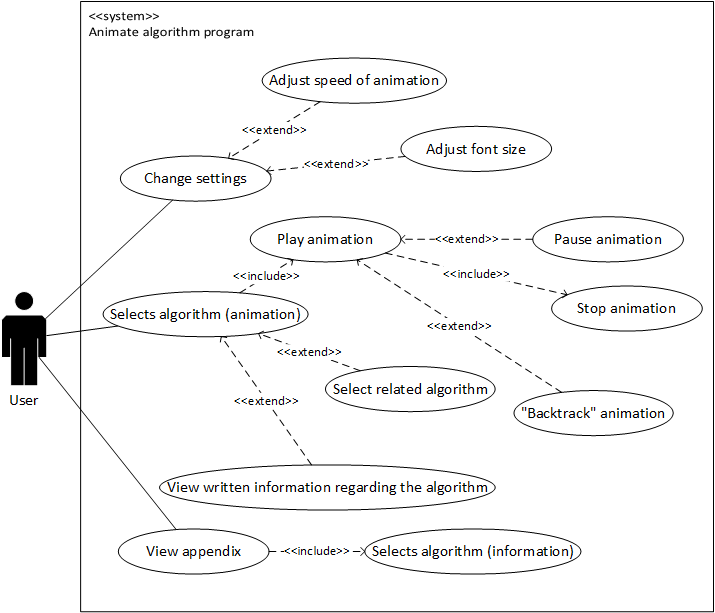
\includegraphics[scale=1]{images/report_images/useCaseDiagram.png}
\caption{The system use case diagram}
\label{useCaseDiagram}
\end{figure}

According to the use case diagram shown on figure \ref{useCaseDiagram}, the user can change the settings of some of the features of the program, such as the speed of the animation, and its font size. This is to ensure that the user will be able to work comfortably within the environment, when the program allows the them to change these features of the program. The user could always revert back to the system's default settings if there is a need to.

Other than the settings, the animation is another feature that would be included within the program. By selecting an algorithm from the list of algorithms, the program will lead the user to the page where the animation of the algorithm resides in. From here, the user can manipulate the animation, by pressing controls such as play, pause, stop and ``backtrack''. The user can also access other algorithms that are \textit{related} to the current one, if they ever wish to do so. If the user clicks on the algorithm from the list of related algorithms, the program then goes to the animation page of the algorithm that was selected by the user.

Other than the settings and the animated feature, there will be an appendix within the program, where the users can view more information about the algorithm. The appendix however will only list the algorithms that are available in the program as animations. Within this feature, the appendix will mainly include a more detailed explanation about the algorithm that is not mentioned in the animation page. The information that can be found in the appendix is expected to contain predominantly texts and images of the algorithm.

\newpage

% --------------- FLOWCHART -------------------
\section{System flowcharts}
In this section, I have included the flowcharts of the program, to display the flow of the system in general, and how decisions controls its following events. 

\subsection{Main flow of the program}
The flowchart below on figure \ref{mainFlowChart} shows the overall flow of the program itself. The three main modules which makes up the program, i.e. change settings, view the animation of algorithms, and the appendix, are grouped in its respective subprocesses. Each subprocess will be described more in detail in sections \ref{sec:flowchartAnimation}, for the animation module, and \ref{sec:flowchartAppendix} for the appendix module.

\begin{figure}[H]
\centering
\hspace*{-1cm}
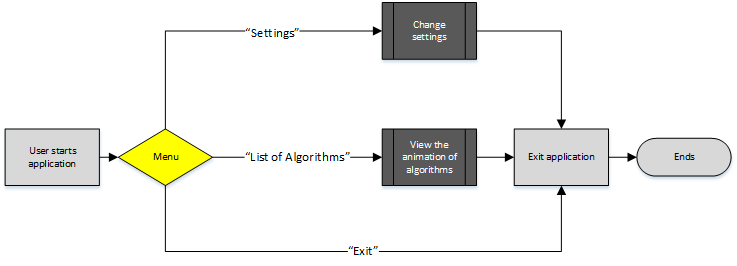
\includegraphics[scale=1]{images/report_images/flowchartMain.png}
\caption{The flowchart of the whole system.}
\label{mainFlowChart}
\end{figure}

On the main flow chart below, the user first starts the application, which then brings them to the main menu. From here, the user can select up to three features they wish to use, which are \textit{Settings}, \textit{List of Algorithms}, and \textit{Appendix}. The user can also choose to exit from the main menu, by selecting \textit{Exit} which then closes the whole application.

\subsection{Flow of the animation module} \label{sec:flowchartAnimation}
The animation module is admittedly the main feature of the program which will be heavily concentrated during the course of the implementation of the project. The user first selects the \textit{List of Algorithms} button, that leads to the animation module. From here, a list of the algorithms are classified between 3 main paradigms and a sorting algorithm into different sections for user feasibility purpose. When the user selects an algorithm they wish to learn more about, the program would lead them to a page where the animation is, and a brief description about the algorithm shown in the \textit{Information} section placed below the animation. 

The program will first prompt the user either to enter their own specific input, or the generate a random value instead. When the user decides to add their own input, there will be a specific limit assigned to the algorithm. If the input exceeds the limited amount, the program will throw an error message to inform user that the input was unacceptable, and requests the user to add an input that does not exceed the assigned limit. On the other hand, if the user selects the \textit{Generate random value} button instead, the program would then generate a random value within the limited amount assigned, and input those value into the animation.

Once an input has been either retrieved, the user then will able to play the animation by pressing the play button. Whilst the animation is at its \textit{playing state}, the user can control the animation by either \textit{pause}, \textit{backtrack}, or \textit{stop} the animation. The state of the animation depends on the type of controls that have been selected by the user. To view the description of each control available in the animation page, below on table \ref{tab:animationControls} that shows the outcome of the animation's state when a particular control button has been selected by the user.

\begin{table}[H]
\caption{The list of animation controls.}
\begin{center}
%\begin{tabular}{cc}
\begin{tabular}{| p{4cm} | p{11cm} |}
		\hline
		\textbf{Control} & \textbf{Description} \\ \hline
		Play & This button simply initiates the animation. This button is only available for use when the animation is either at its initial stage, \textit{paused}, or \textit{stopped}. \\ \hline
     Pause & When a paused button is activated whilst the animation is playing, the animation stops temporarily. The stopped time will be saved, and will continue from that time if whenever the user chooses to play the animation. User can only pause the animation when the animation is being played. \\ \hline
     Backtrack &  This is a unique feature that comes in with the program. As the animation is animated through the use of \textit{iterations}, these iteration values will be counted and stored programmatically. When a user clicks this button, the iteration counter, \textit{i}, will be brought back to the previous iteration, which is \textit{i - 1}. Once it goes back to its previous iteration, the animation will be brought to its \textit{paused} state. From here, the user can press \textit{play}, which will initiate the animation from that particular state. \\ \hline
     Stops &  A stopped button will completely halt the process of the animation. Its final playing state will be discarded once a stop button is selected. \\ \hline
\end{tabular}
\end{center}
\label{tab:animationControls}
\end{table}

\begin{landscape}
\begin{figure}[H]
\centering
\hspace*{-2cm}
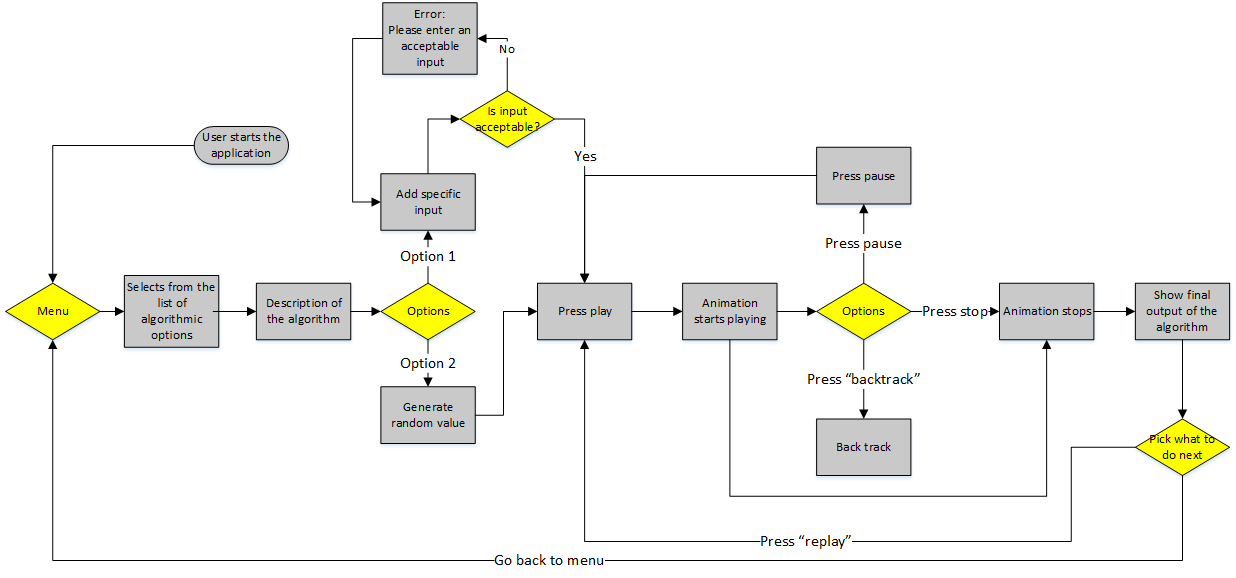
\includegraphics[scale=0.9]{images/report_images/flowchartAnimation.png}
\caption{The flowchart of the animation module.}
\label{flowchartAnimation}
\end{figure}
\end{landscape}

\newpage

\subsection{Flow of the appendix module} \label{sec:flowchartAppendix}
Finally, the last module would be the appendix module, which will contain the supplementary material in regards to the algorithms that are used in this program. This basically lists all the algorithms that are used, and users can select any algorithm within that list to view more information about the algorithm.

\begin{figure}[H]
\centering
%\hspace*{-1.5cm}
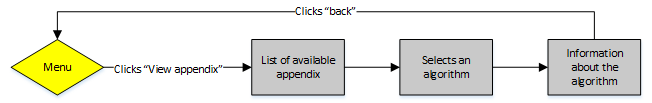
\includegraphics[scale=1]{images/report_images/flowchartAppendix.png}
\caption{The flowchart of the appendix module.}
\label{flowchartAppendix}
\end{figure}

The flowchart on figure \ref{flowchartAppendix} refers to the sequence of events that are involved within the module. First, from the main menu, as when the user selects \textit{View appendix}, the program then brings the user to the list of all the available appendix found in the program. The user then could select the algorithm they wish to find out more about, by clicking one from the list. This will then lead the user to the page that predominantly presents the detailed information in regards to the algorithm in question.

\newpage

% --------------- UI DESIGN -------------------
\newpage
\section{Graphical User Interface design of the system} \label{uiDesign}
\subsection{Program start page}

\begin{figure}[H]
\centering
%\hspace*{-1.5cm}
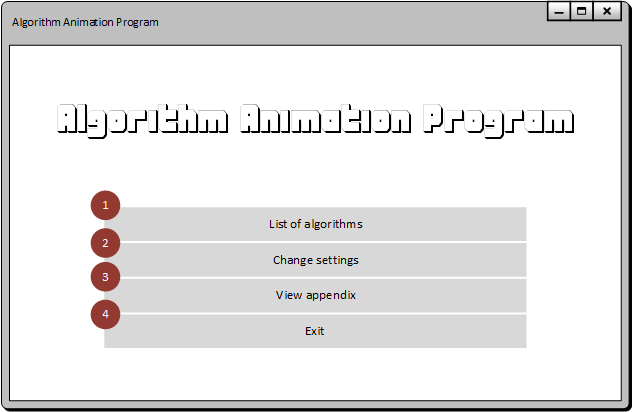
\includegraphics[scale=1]{images/report_images/uiStartWindow.png}
\caption{The start page of the program}
\label{uiStartWindow}
\end{figure}

As the program first initiates, the UI design shown in figure \ref{uiStartWindow} will be the start page of the application. The start page displays the main menu of the application. 

\begin{enumerate}
\item The \textit{List of Algorithm} button leads the user to the list of algorithms. In this list, user can select whatever algorithm they wish to learn. 
\item The \textit{Change settings} button on the other hand, leads the user to a settings page.
\item The \textit{View appendix} page brings the user to the main appendix list, which lists all the algorithms that is shown within the program.
\item Finally, the \textit{Exit} button would close the whole application, if the user selects it.
\end{enumerate}

\newpage

\subsection{Settings page}

\begin{figure}[H]
\centering
\hspace*{-0.5cm}
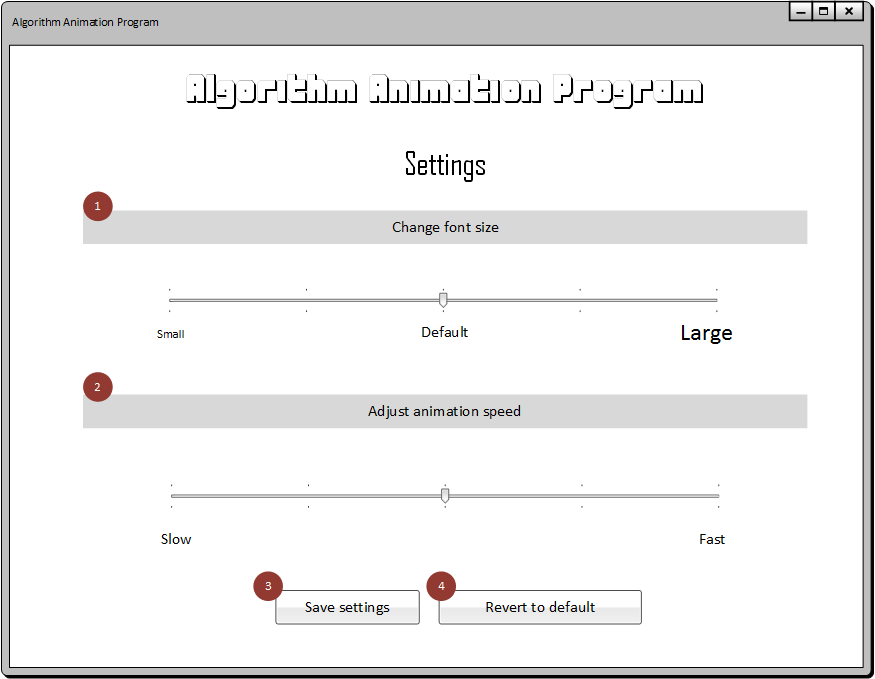
\includegraphics[scale=0.8]{images/report_images/uiSettings.png}
\caption{The settings page.}
\label{uiSettings}
\end{figure}

On the \textit{Settings} page, users can adjust several features of the program, such as the font size, and the animation speed. The reason for having a settings page is to ensure that the users are working in an environment that they are most comfortable in.

\begin{enumerate}
\item One of the features the user can change is the font size. In order to change the font size, the user is to use the slider below. From the leftmost part of the slider is the smallest size of the font, which is size 9pt. The default size on the other hand is 12pt, followed by the largest possible size is 18pt. 
\item Secondly, the user can also change the animation speed. Initially, the animation will be running on a default speed of \todo[color=orange]{find the specific speed of the animation!}. However, if the speed is either too fast or slow for the user, the user could always adjust the speed by sliding to the leftmost bit of the slider for slower speed, and rightmost for a faster speed.
\end{enumerate}

\subsection{List of algorithms page}

\begin{figure}[H]
\centering
\hspace*{-0.5cm}
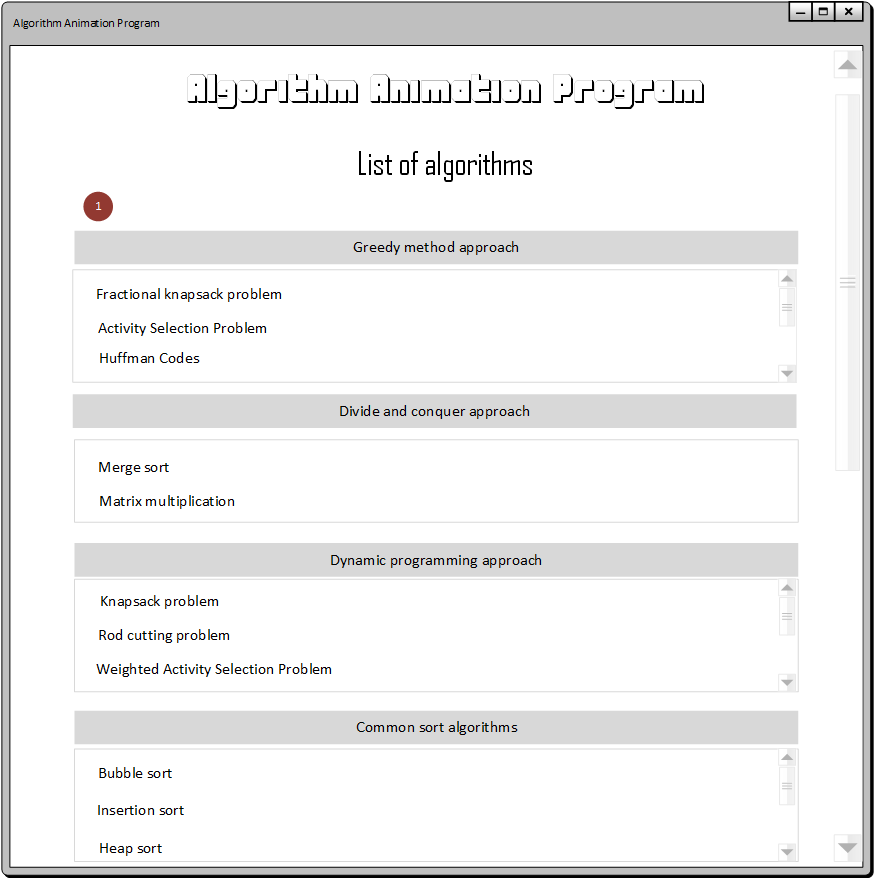
\includegraphics[scale=0.8]{images/report_images/uiListOfAlgorithms.png}
\caption{The page that shows the list of algorithms available for animation.}
\label{uiListOfAlgorithms}
\end{figure}

In this page basically shows the list of all the algorithms that are available in animation. These algorithms are also to be classified between the three main algorithmic paradigms, which are \textit{greedy method}, \textit{divide and conquer}, and \textit{dynamic programming} approaches. Also, another classification would be the sorting algorithms will be included in the list as well.

\begin{enumerate}
\item Shows the list of all the algorithms available. These algorithms are also classified according to its respective algorithmic paradigms. Users can click any of those algorithms displayed in that list if they wish to learn more about them.
\end{enumerate}

\subsection{The page of the animation of the algorithm selected}

\begin{figure}[H]
\centering
\hspace*{-0.5cm}
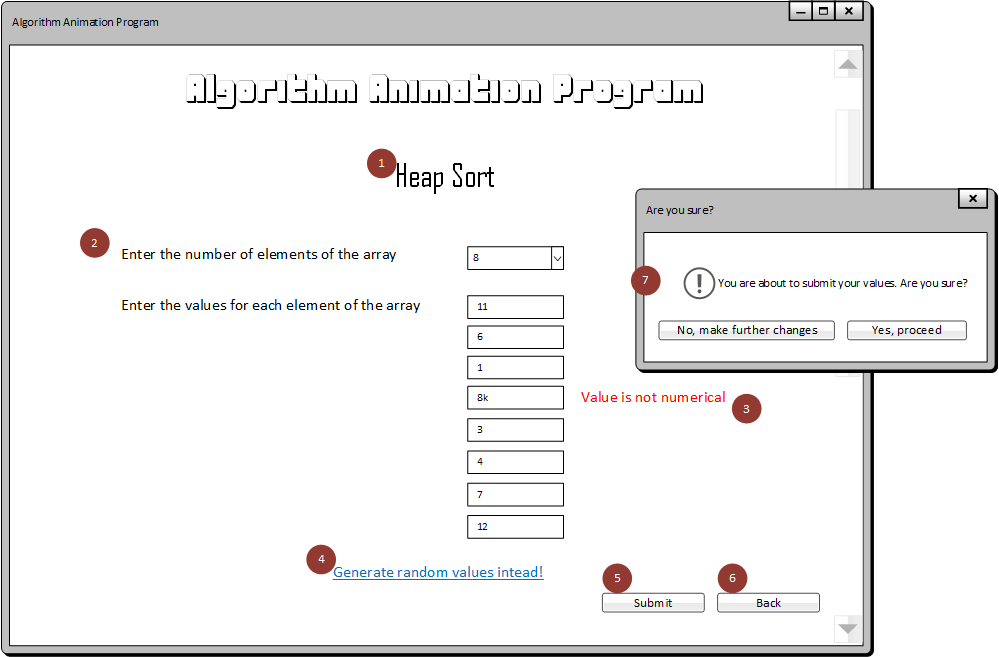
\includegraphics[scale=0.7]{images/report_images/uiInputAnimation.png}
\caption{The page that shows requests the input from the user before starting the animation of the algorithm.}
\label{uiInputAnimation}
\end{figure}

\begin{enumerate}
\item The title of the algorithm in question.
\item The form page of the list of input that is required for the heap sort animation.
\item As all fields are equipped with validation, it will throw an error message in regards to the field if it happens to receive the wrong input. For this case, the user fails to insert a numerical value.
\item Another option instead of adding the user's own input is to generate random values for the animation.
\item This button submits the values and proceeds to the next page, shown in figure \ref{uiAnimation}.
\item This button simply brings the user back to the list of algorithms.
\item This dialog will be prompted once the user clicks the \textit{Submit} button. This is to ensure that the user is happy with the input they have given. From here, if they click \textit{No, make further changes}, the dialog will close, and the page remains the same. If the user clicks \textit{Yes, proceed}, the program will proceed to the next page, which is shown in figure \ref{uiAnimation}.
\end{enumerate}

\begin{figure}[H]
\centering
\hspace*{-0.5cm}
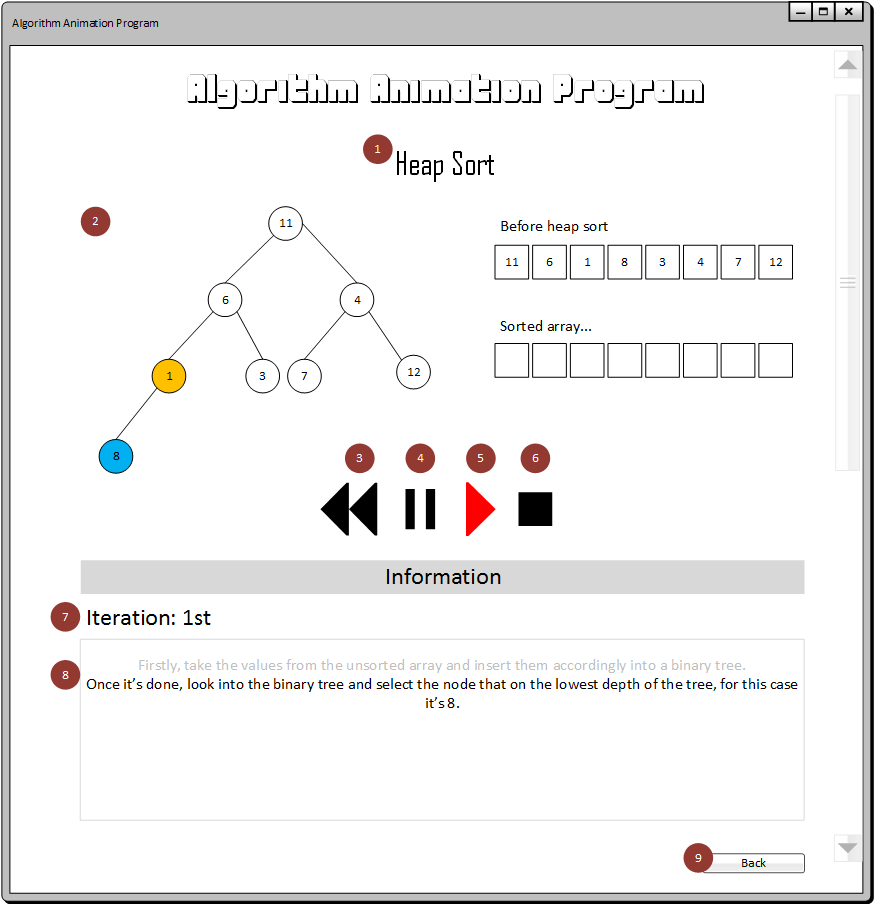
\includegraphics[scale=0.8]{images/report_images/uiAnimation.png}
\caption{The page that shows the animation of the algorithm.}
\label{uiAnimation}
\end{figure}

\begin{enumerate}
\item The title of the algorithm in question.
\item The section of the page where the animation of the algorithm is carried out.
\item The backtrack button.
\item The pause button.
\item The play button. Turns red when the animation is at the \textit{playing state}. This applies to other control buttons as well.
\item The stop button.
\item The number of iteration the animation is currently at. Every time the animation finishes its \textit{main loop}, the iteration counter is added, and it will be displayed here.
\item The area where a written information regarding the animation is displayed. Every time an animation displays something new, a new text block is displayed here, along with the numbers (variables) involved the animation. Once the animation has moved on to the next step, the text mentioned will be greyed out, as the new text will be the one that is emphasized. 
\item The button simply brings the user back to the previous page which would be the main list of algorithms. Whatever that is played in the animation will be discarded.
\end{enumerate}

\newpage

\begin{figure}[H]
\centering
\hspace*{-0.5cm}
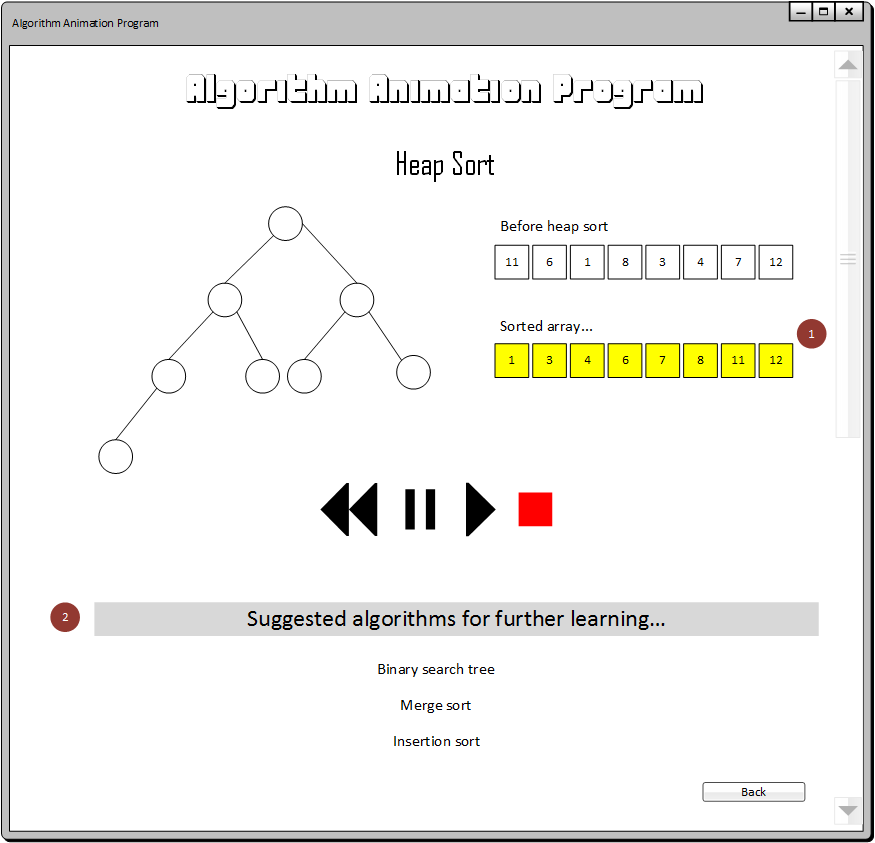
\includegraphics[scale=0.8]{images/report_images/uiAnimationDone.png}
\caption{The page's layout when the animation has finished playing.}
\label{uiAnimationDone}
\end{figure}

\begin{enumerate}
\item The animation stops right when the array has been fully sorted (only applies in sorting algorithms), or in general, has satisfied its respective goal(s). For this example, the sorted array is highlighted in yellow to show that the values in the array has been fully sorted.
\item Secondly, once the animation has ended, it also suggests the user on algorithms that are closely related to the current one for a comprehensive learning experience.
\end{enumerate}

\subsection{The appendix page}

\begin{figure}[H]
\centering
\hspace*{-0.5cm}
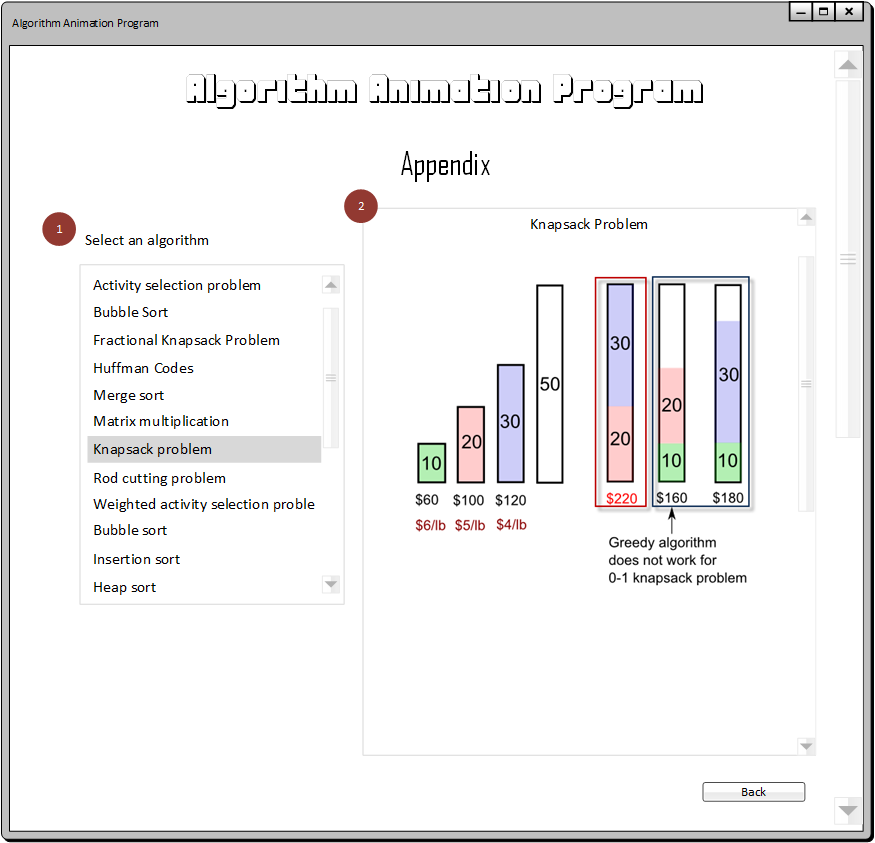
\includegraphics[scale=0.8]{images/report_images/uiAppendix.png}
\caption{The appendix page which lists the algorithms available in the program, which then shows further information regarding the algorithm.}
\label{uiAppendix}
\end{figure}

\begin{enumerate}
\item This section lists all the algorithms available in the program.
\item This section on the other hand displays whatever information about the algorithm selected from the list in no. 1.
\end{enumerate}

\newpage

% -------------- UML Class diagram --------------

\section{UML class diagram}

Show in figure \ref{UMLClassDiagram} is the class diagram of the \textit{Algorithm Animation Program}. The class diagram is a representation of the objects, its attributes, methods, and their relationship amongst others. Whatever is shown in the class diagram will be involved in the construction of the system. 

\begin{landscape}
\begin{figure}[H]
\centering
%\hspace*{-0.5cm}
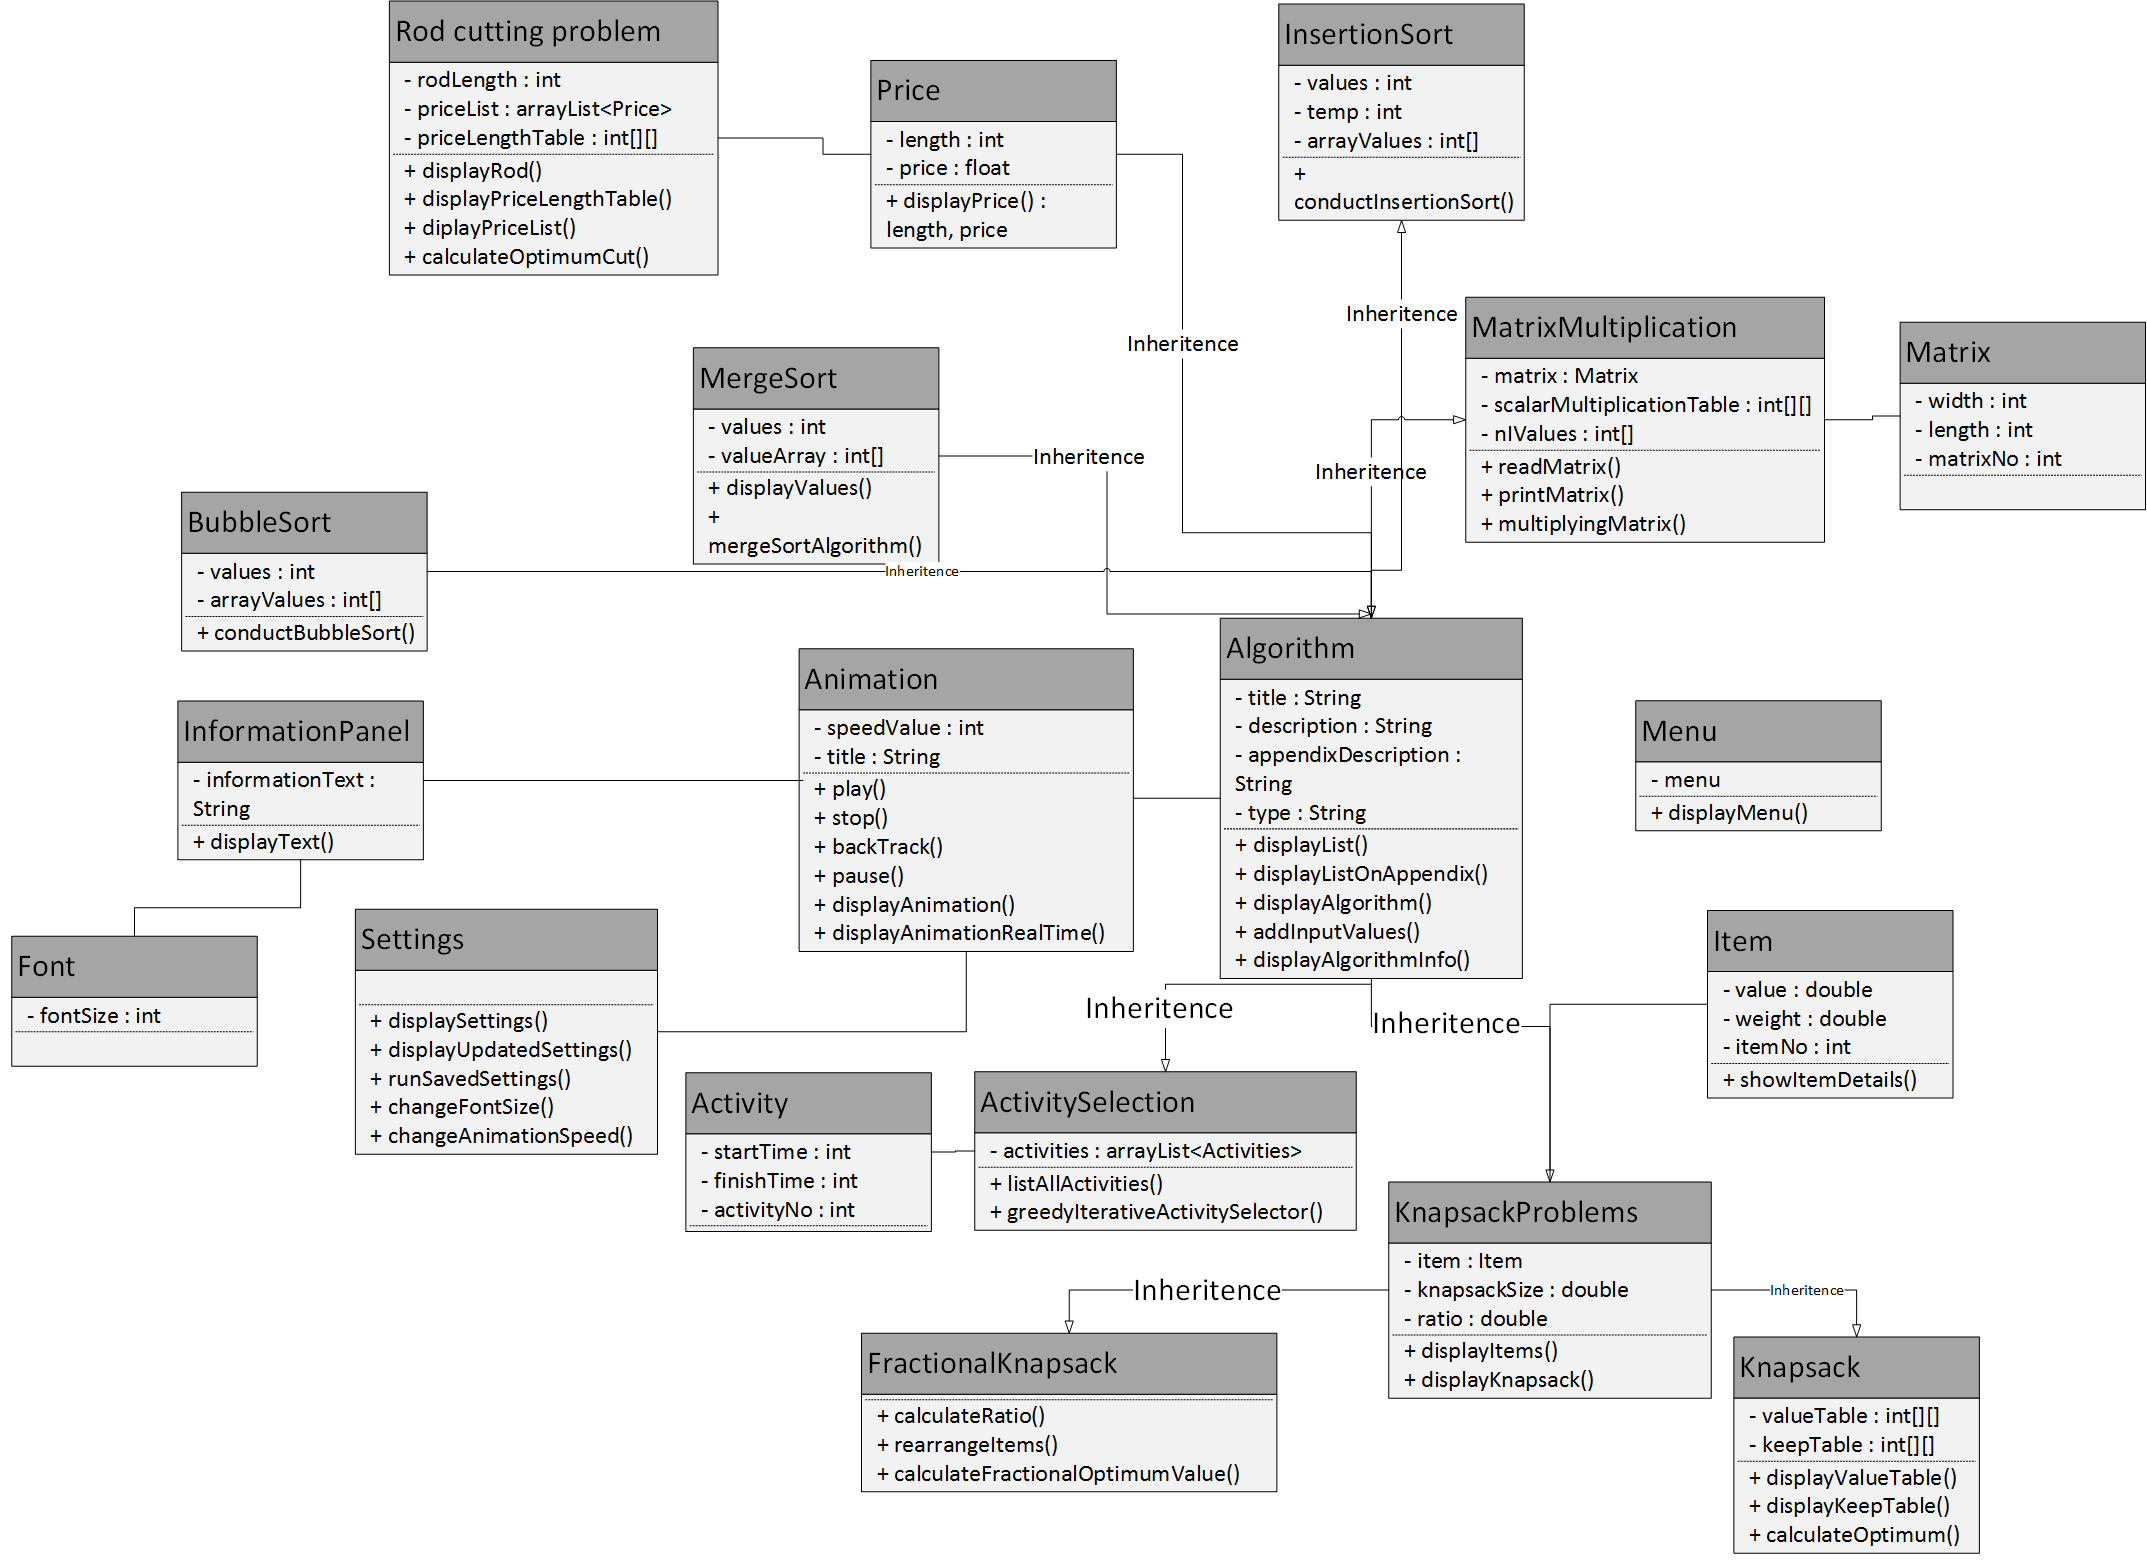
\includegraphics[scale=.37]{images/report_images/UMLClassDiagram.png}
\caption{The UML class diagram for the \textit{Algorithm Animation Program}}
\label{UMLClassDiagram}
\end{figure}
\end{landscape}

\newpage

%--------------- UML Sequence Diagram ----------
\section{UML Sequence Diagram}

Next up, is the sequence diagrams. These diagrams are primarily used to show the interactions between its objects in a sequential order, and the interactions that occur afterwards. The purpose of this diagram is to show in greater detail, compared to the class diagram shown in the previous section (section \ref{UMLClassDiagram}), of what objects that are involved during a particular event. Do take note that these diagrams will be separated between the three main features of the program, the \textit{animation}, \textit{settings}, and finally \textit{appendix}.


\subsection{The animation feature}
The sequence diagram for the animation feature shown in figure \ref{sequenceDiagramShowAlgorithmList}, reveals the interaction between the user and the different objects that are expected to be involved within this feature. First and foremost, as the user initiates the program, the program will display the main menu by executing the \textit{displayMenu()} method. From there, the user selects (for this case) the \textit{List of algorithms} button, which leads the user to the main list of algorithms.

The user then can pick any algorithm they wish to learn from this list. For example, the uses decides to learn how the merge sort algorithm works. So the user clicks the button called \textit{Merge sort algorithm}, which then leads the user to the next page, the input request page, or known as \textit{AlgorithmAnimationInputRequest} according to the sequence diagram in figure \ref{sequenceDiagramShowAlgorithmList}.

Once the values have been inserted, the program proceeds to the animation page by calling out the \textit{displayAnimation()} method, along with the \textit{play()} method that plays the animation. Once the animation is playing, the user can manipulate the animation by using the control buttons such as the \textit{play}, \textit{pause}, \textit{stop}, and \textit{backtrack} button. Each of these controls has its own call of method, and will be called accordingly depending on which control button is pressed. 

If any control button is pressed, the program then calls out the \textit{displayAnimationRealTime()} method. This method predominantly used to run the animations, such as keeping track of the iteration(s) of where the animation is currently at, and also tracks where the timing of the animation is currently at when a control button is clicked. Of course, the latter does not apply to the \textit{stop} button, as the animation will be told to immediately reach to the end once the animation has stopped. 

Once the animation has stopped, either by the user or the animation simply reaches to its own end, the program will then give the user an option of viewing other algorithms that are similar to the one in question, by calling the \textit{getSuggestedAlgorithms()} method. The user can either click one of the suggested algorithms, or choose to go back, which brings them to the main algorithm list.

\begin{landscape}
\begin{figure}[H]
\centering
%\hspace*{-1.5cm}
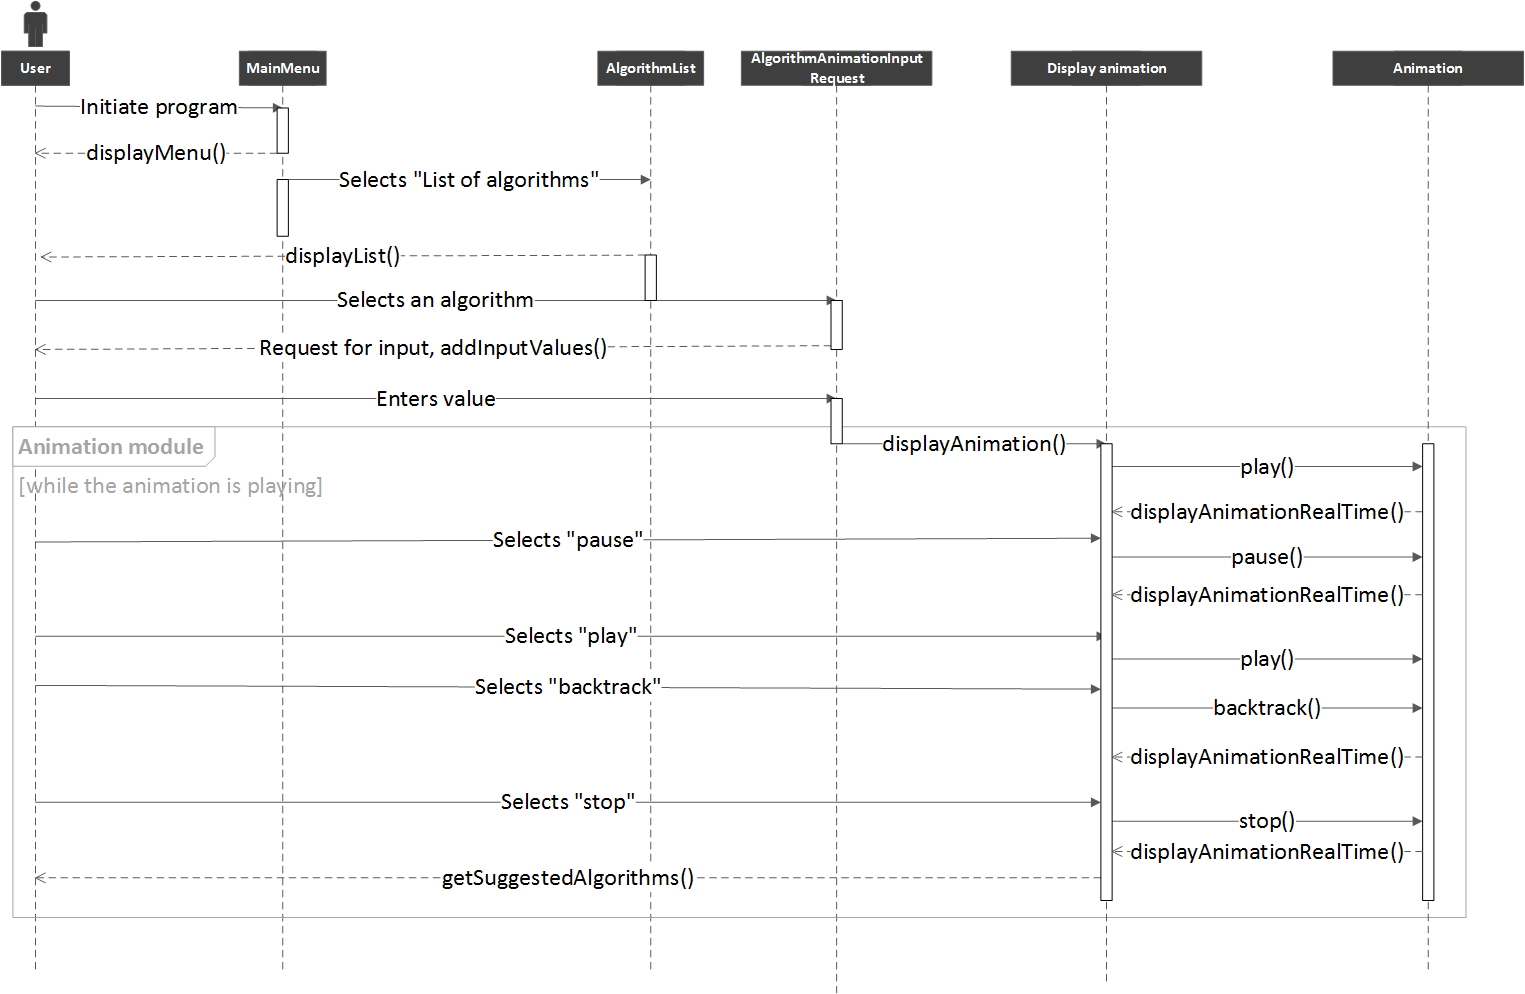
\includegraphics[scale=0.55]{images/report_images/sequenceDiagramShowAlgorithmList.png}
\caption{The sequence diagram of when the user uses the animation feature.}
\label{sequenceDiagramShowAlgorithmList}
\end{figure}
\end{landscape}

\newpage

\subsection{The settings feature}

\begin{figure}[H]
\centering
\hspace*{-1cm}
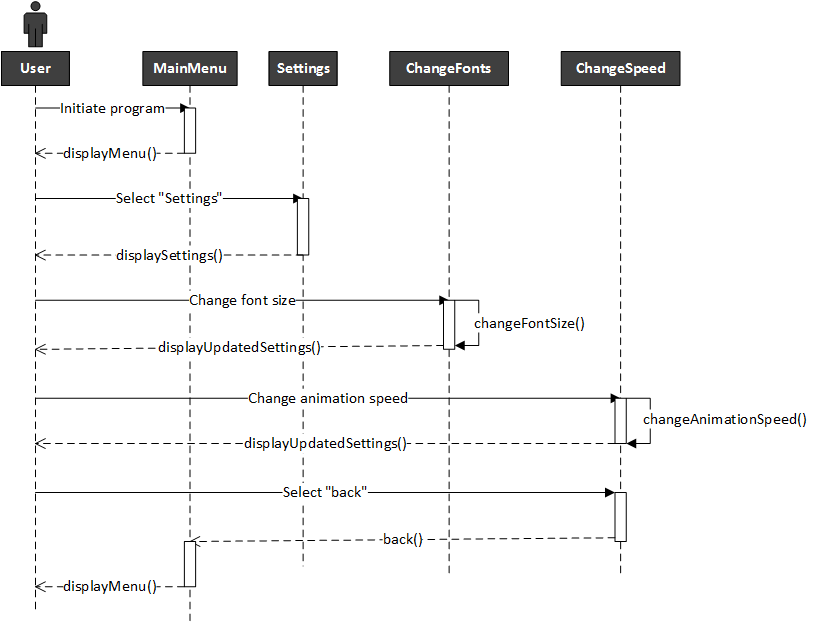
\includegraphics[scale=0.9]{images/report_images/sequenceDiagramSettings.png}
\caption{The sequence diagram of when the user uses the settings feature.}
\label{sequenceDiagramSettings}
\end{figure}

Another feature that is available in the program would be the settings feature. Based on the sequence diagram in figure \ref{sequenceDiagramSettings}, as when the user opens the program, the program will call the \textit{displayMenu()} method to display the main menu onto the client. The user then selects \textit{Settings} button, which leads them to the settings page, which would be called out by the \textit{displaySettings()} method.

Once the user is in the settings page, the user can change features such as the font size and the animation speed. If the user decides to change the font size, the \textit{changeFontSize()} method is being called out. When the method is called, it passes the parameter of the font size chosen by the user, and uses it to make necessary changes to the font size. Once that is done, the program then calls out the \textit{displayUpdatedSettings()} to change the outlook of the program to whatever that is changed. The same applies to when the speed of animation is changed, however this time, the \textit{changeAnimationSpeed()} method is called out instead. 

Once the user is done with changing the settings, they could then press the \textit{Back} button, which leads them back to the main menu. To see the graphical interface design of the settings page, do refer to figure \ref{uiSettings}, on page \pageref{uiSettings}.

\newpage

\subsection{The appendix feature}

\begin{figure}[H]
\centering
%\hspace*{-0.5cm}
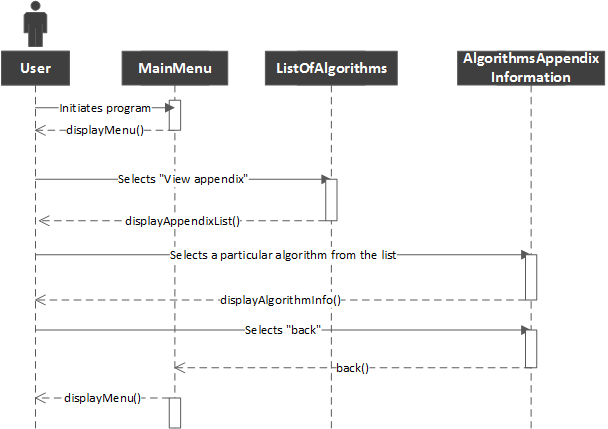
\includegraphics[scale=1]{images/report_images/sequenceDiagramAppendix.png}
\caption{The sequence diagram of when the user uses the appendix feature.}
\label{sequenceDiagramAppendix}
\end{figure}

Last but not least, the appendix would be the other feature that would be available in the \textit{Algorithm Animation} program. From the main menu, the user clicks the \textit{View appendix} button, which calls out the \textit{displayAppendixList()} method, and leads the user to the appendix page. Once the appendix page is displayed, the user could select the algorithm they wish to find out more about, within the list presented on the page. Once the user selects one, the program calls out the \textit{displayAlgorithmInfo()} with the name of the algorithm as the passing parameter, which displays the information available for the algorithm.

When the user is done, the \textit{Back} button can be selected, which leads them back to the main menu. Like before, if you wish to refer to the graphical user interface design of the appendix page, refer to figure \ref{uiAppendix} in page \pageref{uiAppendix}.

\newpage

% ------------- Algorithm animation design ----------------
\section{Algorithm animation designs}
In this section, I will present you the designs of the animations that will be included in the \textit{Algorithm Animation} program. This section is to propose an idea how the animation will look and act like, and to give a guidance on how to develop them during the implementation stage. Alongside with the design of the animation, I will also include a brief description about the algorithm, and whatever is happening within the animation.

Note that I have not included the control buttons in some of these designs. This section is mainly to emphasize the design of the animation of the algorithm in question. If you would like to refer to the design of the actual graphical interface within the animation page, do have a look at section \ref{uiDesign}, on page \pageref{uiDesign} for more details.

\subsection{Fractional Knapsack Problem}
\begin{figure}[H]
\centering
%\hspace*{-0.5cm}
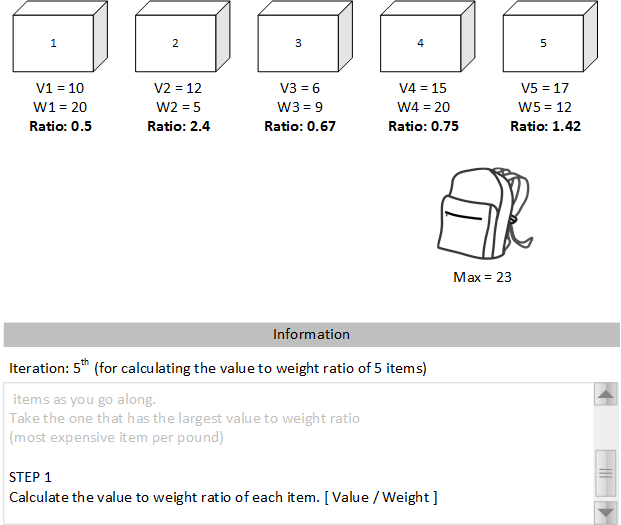
\includegraphics[scale=1]{images/report_images/animationDesignFractionalKnapsackProblem_STEP1.png}
\caption{The animation design of the FractionalKnapsackProblem. This shows the initial state of the animation.}
\label{animationDesignFractionalKnapsackProblem}
\end{figure}

The Fractional Knapsack Problem is one of the algorithms that uses a combinatorial optimisation strategy in which the goal is to fill the knapsack with fractional amounts of items until it reaches to its maximised value. This algorithm predominantly uses the greedy method approach in order to reach to its optimal solution. Within this section, I have included the design of how the animation for this algorithm will turn out to be, along with its descriptions that describes each of the different processes that happens during the play time of the animation.

The graphical interface of the Fractional Knapsack Problem algorithm shown in figure \ref{animationDesignFractionalKnapsackProblem} is the initial state of the animation. The animation consists of the items, which are represented in cubes, along with its values, i.e. weight and value of the item. Other than the items, there will also be an image of a rucksack that represents the knapsack. The knapsack has its max weight, which is the maximum amount of weight it can possible carry, and the current weight it is carrying now.

The next step of this animation shown in figure, is simply to follow the process of the animation. In this design, the animation is currently at the stage where it needs to calculate each of the items' value to weight ratio. The animation simply adds another value to each of those items called \textit{Ratio}, that shows the results to the calculation. Next would be the part of the animation is when the items are re-arranged according to their value to weight ratios.

Once the items are finally arranged, it is now time to add the items into the knapsack. The animation will represented that by dragging the item in its current iteration next to the knapsack. An arrow will then appear next to the item to represent the act of adding the item into the knapsack. When the item in question is added into the knapsack, there will be a change on the \textit{Current weight} value. 

There is an exception to this animation, that the knapsack, can no longer contain the total weight of the item in question. So, the animation program will inform the user, under the information section, that it can't insert the whole of item in question. This proceeds the animation to add fractions of the item instead, and doing a simple calculation (ratio * amount of weight left in the bag) along it as well. You can clearly see this calculation clearly above the arrow.

As when the calculation is complete, and the knapsack's current weight has reached to its max weight, the animation then comes into a conclusion. The conclusion of this algorithm is that the knapsack is finally full, and the total value that the knapsack has achieved is displayed as well. Afterwards, the animation stops here. 

\newpage

\lstinputlisting[frame=single, caption=The psuedo code of the fractional Knapsack Problem, label={fractionalKnapsackProblem}]{codes/fractionalKnapsackProblem.java}

The psuedo code of the fractional knapsack problem, shown in listing \ref{fractionalKnapsackProblem}, is basically the construction of how the algorithm will be put to work during the implementation phase. First the algorithm declares the arrayList of \textit{Item} objects, where an \textit{Item} object will have its attributes such as weight and value. The arrayList will store the list of items, which the user has declared on the input page before the animation starts.

Moving on, the algorithm will then calculate each of the items' value to weight ratio. Using those values, the algorithm then sorts the items out, from the item with the largest value to weight ratio, to the one that has the least. From here, the algorithm starts picking the first item from the list, and adding it into the knapsack. However before doing so, the algorithm checks if there is any space left for the knapsack to take in, by comparing the whole weight of the item to the amount of capacity left the knapsack is able to take in. If there is enough space, the algorithm takes in the whole item, otherwise, it starts adding each amount of fraction it is able to take before the knapsack capacity reaches to its full amount. When that happens, the algorithm ends.

\subsection{Knapsack Problem}

The Knapsack Problem is quite similar compared to the Fractional Knapsack Problem. However for this problem, you can only take the whole item and leave the rest if there is no space left in the knapsack, instead of taking items fractionally until the knapsack is full. Despite a minor change in the constraints of this problem, the approach to the knapsack problem is very different to the fractional one. Instead of utilising the greedy method like we would do for the fractional, this requires us to use the dynamic programming approach instead. Because of this, the animation needs to add another feature, and this will basically be applied to all algorithms that uses the dynamic programming approach as well: tables.

\begin{figure}[H]
\centering
%\hspace*{-0.5cm}
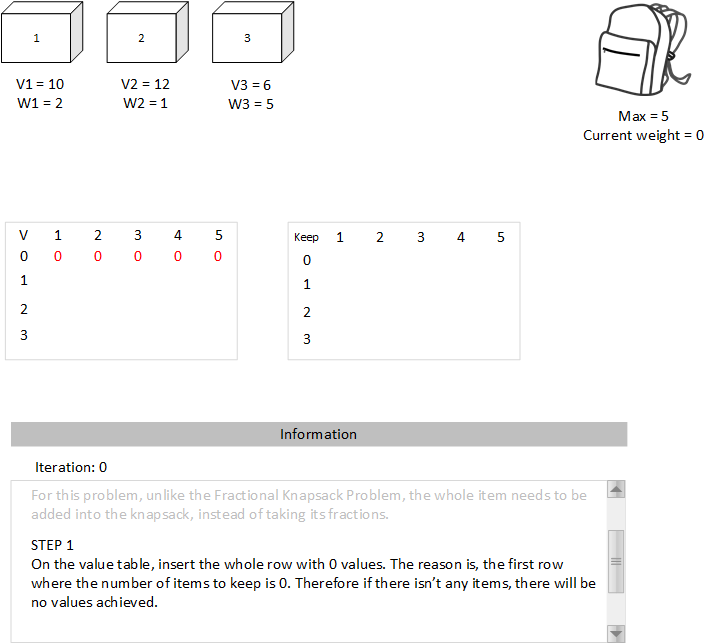
\includegraphics[scale=0.7]{images/report_images/animationDesignKnapsackProblem_STEP2.png}
\caption{The initial state of the animation design of the Knapsack Problem. It shows that it is describing what the tables are.}
\label{animationDesignKnapsackProblem}
\end{figure}

As when the animation of the knapsack problem starts (refer to figure \ref{animationDesignKnapsackProblem}), few description which describes about the tables will be displayed during the animation's initial play time. Those descriptions in the yellow coloured callouts are placed around the table to describe its purpose, in order for the user to understand what they are before the actual algorithm starts. These texts will remain here for about a 30 seconds, before proceeding to the next state.

Included in this animation, other than the ones mentioned before, are the cube figures which represent the items. Along with them are its attributes, which are their respective value they are worth, and their weight. Next to it is an image of the knapsack. Show below it is its maximum capacity, and the current weight it is holding. For its initial state, the current value is always 0.

Within the \textit{Information} section, there will also be a brief description of what the algorithm is, and how is it different from the Fractional Knapsack algorithm. 

After the explanation phase has completed, the algorithm of the knapsack problem begins. The algorithm begins by applying the sum of values obtained on the first row of the \textit{value table}. Since on the left side of the table is 0, meaning that there are no items selected, all the values are returned as 0 for the first row. The texts that are inserted into the table are turned red, simply to let the users know where to look in the animation. The values are added into the \textit{keep table} as well after adding those values into the \textit{values table} previously.

As the animation proceeds to the second row, where the animation loops by doing the same thing previously on the first row. It refers to the top column, which is the weight of the knapsack to carry, which is highlighted with a green circle. Followed by the spot where the animation needs to compute the value for, which is highlighted with a red circle. 

Once filling up the \textit{value} and \textit{keep} table is completed, the algorithm looks through the keep table from the most bottom right hand side, to find out which item to keep. If the value is 1, it means that the item along that row is kept, and the total weight of the knapsack will be subtracted from the item. Do this along the column which is the maximum possible amount of capacity of the knapsack, in this case 5, until either the knapsack is full, or can no longer take in any more items. Finally once it has done that, show the total value (most optimum value you can achieve) that is taken away from the knapsack.

\lstinputlisting[frame=single]{codes/knapsackProblem.java}
\todo[color=yellow]{describe the psuedo code}

\newpage

\subsection{Activity Selection Problem}

In the Activity Selection Problem, you are given a set of activities, where each have its respective starting and finishing time. Within this set of activities, the goal is to find the most number of activities that can run without interrupting each other. This algorithm uses the greedy method approach in order to find the optimum set of activities. 

\begin{figure}[H]
\centering
%\hspace*{-0.5cm}
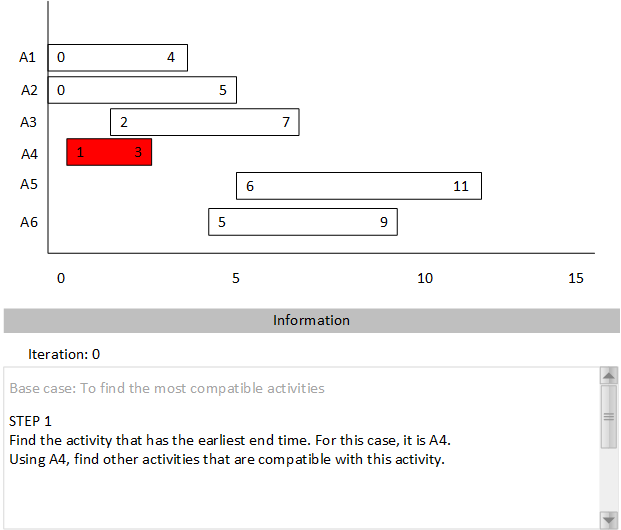
\includegraphics[scale=0.9]{images/report_images/animationDesignActivitySelectionProblem_STEP1.png}
\caption{The animation design of the Activity Selection Problem.}
\label{animationDesignActivitySelectionProblem}
\end{figure}

Shown in figure \ref{animationDesignActivitySelectionProblem}, is the initial stage of the activity selection animation during its starting phase. During this phase, the animation starts off by explaining parts of the diagram, using the bright yellow callouts. Along with it, there is a further explanation about the objective of the algorithm within the information section below.

Once the explanation phase is done, the animation carries on by initiating the activity selection problem algorithm. First, it selects the activity with the earliest end time, and highlights it red. Once the activity has been chosen, it goes on by finding the other activities within the list that is incompatible with the chosen activity. These incompatible activities are then removed from the list of activities, and are greyed out in the animation to show that they are removed. Once there aren't any more activities left in the list of activities, the optimal solution to the problem has been finalised. This is when the animation ends. 

\newpage

\lstinputlisting[frame=single]{codes/activitySelectionProblem.java}
\todo[color=yellow]{describe the psuedo code}

\newpage

\subsection{Merge sort}

\begin{figure}[H]
\centering
%\hspace*{-0.5cm}
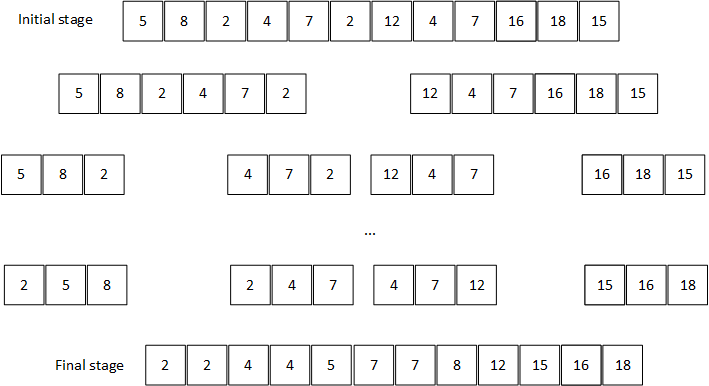
\includegraphics[scale=0.9]{images/report_images/animationDesignMergeSort.png}
\caption{Merge sort animation design.}
\label{animationDesignMergeSort}
\end{figure}

The merge sort algorithm is basically one of the sorting algorithms that uses the divide and conquer method to sort the contents of the array of values. The animation for the merge sort algorithm will emphasize mainly on the idea of a divide and conquer, which is one of the three algorithmic paradigms. 

On the input page for the merge sort algorithm, will be the number of elements in array, followed by the values for each element of the array. The animation for this algorithm will be made simple, as you can see in figure \ref{animationDesignMergeSort}. First, is to have squares that represents each element of the array. These squares will initially be set next to the other squares with values clearly shown on them.

As when the animation starts, the animation will clearly show the division it makes to divide the array into 2 parts, each side with an equal amount of elements to the other side (unless if the total number of elements is an odd number, then one side will have one more element than the other). The animation will keep on doing this until each of the elements divided will be left to one each. After which, the animation will proceed in taking the first element from the unsorted list, sorts and drags it down to another tier, and do the same for the rest until all the elements are sorted and merged as a whole. The animation then concludes by showing that it is finally sorted, and ends here.

\newpage

\lstinputlisting[frame=single]{codes/mergeSort.java}
\todo[color=yellow]{describe the psuedo code}

\newpage

\subsection{Matrix multiplication}

\begin{figure}[H]
\centering
%\hspace*{-0.5cm}
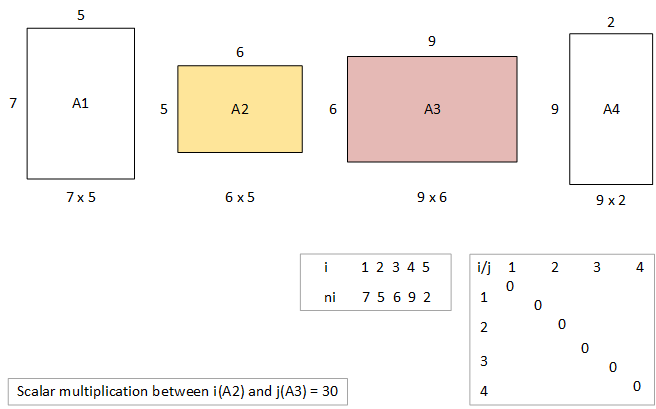
\includegraphics[scale=0.9]{images/report_images/animationDesignMatrixMultiplication.png}
\caption{Merge sort animation design.}
\label{animationDesignMatrixMultiplication}
\end{figure}

The matrix multiplication problem is classified under the \textit{optimisation problem}, that will be available in animation. This problem simply shows the algorithm on finding the most efficient way to multiply two or more matrices together, and using dynamic programming in order to find the solution. 

The input page for the animation will consist of the number of matrices to compute and the size of each of those matrices. There will be some constraint when it comes to selecting the size of the matrix however, is that, the next matrix will need to have one of its sides to be the same value as one of the sides the first matrix as well, which is a basic rule for two matrices to be multiplied with one another.

On the animation itself, it will present each matrix in a rectangular shaped figures, depending on the size that was given during the input stage. On top of each matrix will also be an identifier, which format is \textit{Mi}, \textit{i} being the number of the matrix in the list. Below each of the rectangles will show the size of the matrix, which format goes as \textit{widthSize * lengthSize}, in order to depict the size of each rectangles.

During a part of the animation, the algorithm will pick the values for \textit{i} and \textit{j}, which are the values between the 1, the first matrix, and N, where it is the number of the last matrix in the list. Between these two values, there will also be \textit{k}, which is going to be used to compute the most efficient \textit{split} to be made, in order to achieve the minimal amount of scalar multiplications between the two lists of the matrices. In every iteration of the algorithm, the animation is to use \textit{k} as a splitter, and between the two parts of the list, find the minimum amount of scalar multiplications needed. And once the minimum has been found, the algorithm will conclude its answers, and ends.

Since this problem uses dynamic programming, there is a need to add a table that goes with the animation as well. This table is what I call the \textit{i and j} table, which is a two dimensional array that makes up the size of \textit{i} and \textit{j}. This table is used to store the result of the scalar multiplications between the size of the matrices, and is used to find the most efficient solution for the problem. 

\newpage

\lstinputlisting[frame=single]{codes/matrixMultiplication.cs}
\todo[color=yellow]{describe the psuedo code}

\subsection{Rod cutting problem}

\begin{figure}[H]
\centering
%\hspace*{-0.5cm}
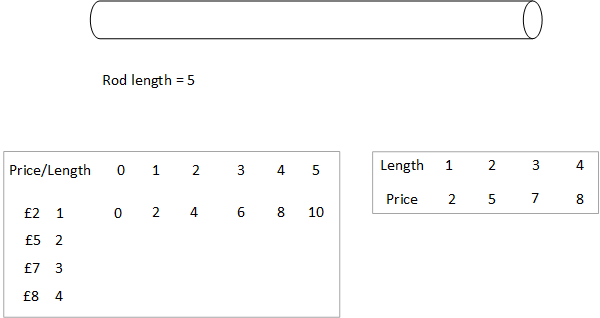
\includegraphics[scale=0.9]{images/report_images/animationDesignRodCuttingProblem.png}
\caption{Merge sort animation design.}
\label{animationDesignRodCuttingProblem}
\end{figure}

The rod cutting problem is another one of those algorithms that uses the dynamic programming strategy. The problem consists of a rod, which is a x amount of length. Along with it, there is a table of prices, selling for a certain amount for a certain amount of length. Using some sort of a strategy (for our case, an algorithm), find the best cuts of the rod of x length, in order to get the most value out of it.

In the input page for the rod cutting problem, would have the input for the length of the rod, and the prices for each length of the rod. When the input is inserted, the animation starts by showing the image of a rod, with the length assigned to it. Below it as well are two tables, one of them, the \textit{Price/Length} table, is the table that is used to calculate the price earned for selling the rod at a certain length. This table will be filled along the way during the course of the animation. The other table is the \textit{price table}, which lists the set of length and its prices. 

The algorithm ends when the \textit{Price/Length} table is fully filled, and the optimum cut is retrieved from the table. The animation will then conclude the optimum price for the particular problem before it terminates.

\todo[color=yellow]{psuedo code}

\newpage

\subsection{Bubble sort}

\begin{figure}[H]
\centering
%\hspace*{-0.5cm}
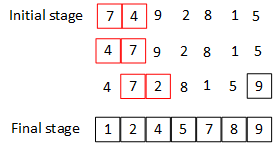
\includegraphics[scale=1.5]{images/report_images/animationDesignBubbleSort.png}
\caption{Merge sort animation design.}
\label{animationDesignBubbleSort}
\end{figure}

The bubble sort is one of the sorting algorithms that I will include in this program, classified under the \textit{Sorting algorithms} section. It is a simple algorithm that compares each adjacent pair, and swaps with one another, left side is the smaller value, whilst the right side is the larger value. The algorithm keeps doing so until the whole list is fully sorted.

For the input page, the values that the program will take before starting the animation would be, the size of the array, and the values for each of the elements in the array.

The animation for the bubble sort algorithm will show the list of values, arranged accordingly to the input that was given by the user, or the random generator. These values are shown basically depict each of the element of the array, and the animation will show clearly that each of them will be swapped with the value next to itself clearly when it is its time to swap. Once the largest value in the list has moved all the way to the right side of the array, a black border will surround it, indicating that the position for this element has been finalised. The animation will come to an end, once all the elements have its own black border. The animation then concludes that the array of values have been sorted, and will stop itself then.

\newpage
\todo[color=yellow]{description about the psuedo code}
\lstinputlisting[frame=single]{codes/bubbleSort.java}

\newpage

\subsection{Insertion sort}

\begin{figure}[H]
\centering
%\hspace*{-0.5cm}
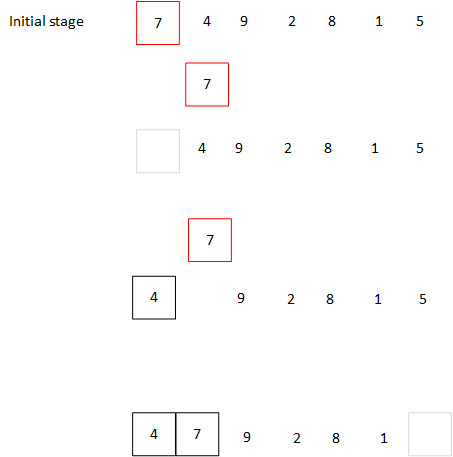
\includegraphics[scale=0.9]{images/report_images/animationDesignInsertionSort.png}
\caption{The insertion sort animation design.}
\label{animationDesignInsertionSort}
\end{figure}

The input page for the insertion sort will be very similar to the input page for the bubble sort. However, of course, the animation of the insertion sort will be different compared to it. At the initial stage, as seen in figure \ref{animationDesignInsertionSort}, the animation shows the values, where these values represents each element in an array. As the animation begins, the first value from the left will be highlighted with a red bordered square, and then``pulled out'' from the main array. This value is then used to compare with the values from the left side, values which are in the black bordered square. The black bordered square is basically to represent the values that the algorithm had gone through, and are sorted. Once the value in the red square has found its place within the values within the black border, the red box for that value changes to black. Then, the next unboxed value will be pulled out the following after.

\lstinputlisting[frame=single]{codes/insertionSort.java}
\todo[color=yellow]{describe the psuedo code}

\newpage

%\subsection{Heap sort}

%Heap sort is another one of the sort algorithms that will be included in the \textit{Algorithm Animation Program}. Unlike the other two sorting algorithms mentioned above, there is a different feature about the heap sort, is that it makes use of a binary tree to create an array of \textit{heap}, followed by using the \textit{heap} array to sort the contents found within it. Another convenient feature about heap sort algorithm  is that, when it comes to sorting, there isn't a need for an additional temporary array. All it requires is the memory that is already given to it (the array of values), and swap the values within the array strategically before sorting them out.

%Like the other sorting algorithms, the input page for the heap sort will be the same. The animation for the heap sort on the other hand, will consist of the list of values in each square, which represents the values found in the elements of the array. The animation will also include the binary tree, which will show in a step by step basis on how, the values from the initial array, is inserted into the tree and finally from that tree, to create a \textit{heap} array. And then of course from there, the animation would also show how the values in the \textit{heap} array is sorted. As when the animation is showing how the binary tree is being applied to, the animation will also show the process of value swapping in the initial array as well. Once the values are sorted, the animation will conclude that that the array has been sorted before stopping.

% ------------- EVALUATION LIST -----------------
\section{The Evaluation Design}

% what are the criteria from the system
% 1 - usability
% 2 - comprehensive
% 3 - correctness

The evaluation will asses on the three main criteria that will be used during the assessment phase, which are \textit{usability}, \textit{comprehensiveness}, \textit{correctness}. The term \textit{usability} plainly refers to the ease of using the program. There are a few pointers for the software to achieve this, which involve in easy installation process, the intuitiveness of its graphical interface, efficient, and its interface is easy to navigate around with and learn.

The next criteria that will be assessed during the evaluation would be the \textit{comprehensiveness} of the program. Since this software is meant to be educational, the software needs to take conscientious measures in making the animation to be easily understood by students, who either have no knowledge or little prior knowledge on the particular subject. Within this criteria, the animations in this program needs to be easily understood, by giving sufficient amount of information that goes hand in hand while the animation is being played. With these two working together, the content that are provided needs to be relevant. These construction of the content that has being displayed are also expected to be clear and concise, and would be easily understood within a short period of time. 

The last criteria that needs to be assessed during the evaluation would be the \textit{correctness} of the contents that is provided in the software. This is another important criteria that needs to be assessed during the evaluation, especially for an educational based software, as it is important for the \textit{Algorithm Animation Program} to sustain the correct depiction of the algorithms shown in the program. 

\subsection{Testers who will be involved during the evaluation}
% who will be involved during the evaluation
There will be a need to include two different sets of groups of testers when it comes to the evaluation of this software. The first group will be involving in computer science students, who either have no knowledge in to having basic knowledge in regards to algorithms. The reason why this group will be used to assessed the program is that they will mainly be assessing the usability and the correctness of the program. Since they have no to little knowledge regarding the topic, it is up to them to see if they have managed to achieve any form of understanding after using the program. The measurement of their understanding will able to show the amount of effectiveness in representing the animations. If they manage to do so, it will show that the representation of the animations are effective.

The second group of testers on the other hand, would involve in students, or lecturers who have an extensive knowledge in algorithms. This group will primarily focus on assessing the validation of the animations that are presented to them. With the help of this group of testers, their feedback will ensure that the animations portraying the algorithms correctly, and if not, state in the evaluation form on what are the areas that are portraying the algorithms incorrectly. They will also assess the correctness of the information that comes with the animation as well, and see if the correlation between the information and animation is relevant and valid. Using their feedback will help me in locating the specific errors found within the animation and its information, and rectifying them.

\todo[color=pink]{I left it off here}

% what testing will be carried out
\todo[color=yellow]{anything to write for what kind of testing to be carried out?}

\subsection{The design of the evaluation form}
Below in table \ref{table:evaluationFormDesign}, I have included the software evaluation form that is expected to be filled out with feedback from the users who will be testing the software. The form includes in defining each criteria, any sub-criteria that comes along with it, and the notes that is explained in plain language on what each of those criteria means. Which then follows by a series of questions that are involved within each criteria, which the testers are expected to fill their feedback in. 

What is expected from the evaluation form is that users are expected to fill in with open ended answers in each sections of the form, describing about their experiences when it comes to using the software. It is also expected of me to obtain feedback, such as what is good or aspects that is lacking in the program. Of course, the users are to give the feedback of the software based on the criteria that they are assessing from, which would definitely gives me a better sense of direction when there is the need to improve on the software. Of course, afterwards, the form allows the users to give any additional feedback if there is a need to. This might be useful, as it might fill in the gaps that I have missed in the criteria based assessment.

\begin{table}[H]
\caption{The design of the evaluation form that will be used for the criteria based assessment.}
\begin{center}
%\begin{tabular}{cc}
\begin{tabular}{| p{8cm} | p{8cm} |}
		\hline
		\textbf{Criteria} & \textbf{Yes/No, supporting feedback} \\ \hline
		\multicolumn{2}{| l |}{\centerline{\textbf{Usability}}}\\ \hline
		Is the program easily understood in terms of usage?  & \\ \hline
		Is it easy to navigate around the program? & \\ \hline
		Can you see the images displayed in the program clearly? & \\ \hline
		Can you see the animation displayed clearly? & \\ \hline
		Is the interface of the program easy to use?  &   \\ \hline
		
		\multicolumn{2}{| l |}{\centerline{\textbf{Comprehensiveness}}}\\ \hline
		Do you understand the general structure of the algorithms presented in the program? & \\ \hline
		Do you understand how each of the algorithms work? List the ones that you understand and the ones you don't. & \\ \hline
		Was it easy for you to understand that the animations are trying to portray? & \\ \hline
		What do you think about the display of the animations in general? & \\ \hline
		Are the information that comes with the animation can be easily understood? & \\ \hline
		Are the information that comes with the animation relevant to the animation? & \\ \hline
		
		\multicolumn{2}{| l |}{\centerline{\textbf{Correctness}}}\\ \hline
		Are the representation of the animations for the algorithms it is portraying correct?  & \\ \hline
		Are the information displayed whilst the animation is playing correct? & \\ \hline
		
		\multicolumn{2}{| l |}{\centerline{\textbf{Other feedback}}}\\ \hline
		Are there any thing that is good in the program? & \\ \hline
		Are there any that is lacking? & \\ \hline
		What do you think that needs to be improved in the software? & \\ \hline
\end{tabular}
\end{center}
\label{table:evaluationFormDesign}
\end{table}

